\documentclass[20pt,landscape,a4paper,footrule]{foils}
\usepackage{solido-network-slides}


% 
% Arrangement:	Penetration testing I - basale pentest metoder og introduktion

% Penetration testing IV - cryptography og cracking

% Kryptografi er en forudsætning for en stol del af vores IT-sikkerhed, men hvad er sikkert? Vi gennemgår forudsætningerne og nogle af de mest almindelige værktøjer til at sikre og knække kryptering. Vi bruger tidligere knækkede algoritmer som eksempler og udfra denne viden opnår vi erfaring som tillader os at vælge hvilke protokoller vi fremover vil benytte til at sikre os. Dette kursus sigter mod at deltagerne efterfølgende vælger de rigtige metoder og kryptering til at sikre systemer og data.

% * Password cracking
% * Wireless cracking / WPA cracking
% * Fuld disk kryptering - forudsætninger og eksempler på fejl
% * GPU og FPGA cracking
% * OpenSSL / LibreSSL - heartbleed som eksempel
% * Tilfældige tal og PRNG Debian
% * IPsec, OpenVPN og andre VPN teknologier, PPTP
% * OPsec



\begin{document}

%\slide{}

\mytitlepage
{Penetration testing IV\\cryptography og cracking}

%\begin{alltt}
%\tiny 
%\centerline{$Id: pentest-I-foredrag.tex,v 1.2 2007/10/04 12:17:42 hlk Exp $}
%\end{alltt}



\LogoOn

%\dagsplan


\slide{Formålet idag}

\hlkimage{10cm}{Encrypt_all_the_things.png}

\begin{list1}
\item Introducere nogle almindelige protokoller og deres krav
\item Introducere basale penetrationstest værktøjer indenfor kryptografi
\item Skabe en grundig forståelse for praktisk anvendelig kryptografi
\end{list1}

\slide{Generic advice}

Recommendations \hlkrightimage{8cm}{Encrypt_all_the_things.png}
\begin{list2}
\item Lock your devices, phones, tables and computers
\item Update software and apps
\item Do NOT use the same password everywhere
\item Watch out when using open wifi-networks
\item Multiple browsers: one for Facebook, and separate for home banking apps?
\item Multiple laptops? One for private data, one for work?
\item Think of the data you produce, why do people take naked pictures and SnapChat them?
\item Use pseudonyms and aliases, do not use your real name everywhere
\item Enable encryption: IMAP{\bf S} POP3{\bf S}
  HTTP{\bf S} TOR OpenPGP VPN SSL/TLS
\end{list2}


\slide{Stop watching us!}

\hlkimage{20cm}{access-now.png}

\slide{Appropriate paranoia}

\hlkimage{15cm}{paranoia-definition.png}

Source: google paranoia definition

\slide{Face reality}

From the definition:
\begin{quote}
suspicion and mistrust of people or their actions {\bf without evidence or justification}.
{\bf "the global paranoia about hackers and viruses"}
\end{quote}

\begin{list1}
\item It is not paranoia when:
\begin{list2}
\item Criminals sell your credit card information and identity theft
\item Trade infected computers like a commodity
\item Governments write laws that allows them to introduce back-doors - and use these
\item Governments do blanket surveillance of their population
\item Governments implement censorship, threaten citizens and journalist
\end{list2}
\end{list1}

\vskip 1cm
\centerline{You are not paranoid when there are people actively attacking you!}


\slide{Credit card fraud and identity theft statistics}

\hlkimage{19cm}{credit-card-fraud.png}

{\small Source: 
\link{http://www.statisticbrain.com/credit-card-fraud-statistics/}}


\slide{Identity theft statistics}

\hlkimage{19cm}{identity-theft-stat.png}

{\small Source: 
\link{http://www.statisticbrain.com/identity-theft-fraud-statistics/}}


\slide{Use protection - always}

\hlkimage{14cm}{protect-from-governments.jpg}
%{\LARGE Protecting yourself against criminals or the government is the same thing!}

\slide{A vulnerability can and will be abused}

What if I told you:

{\Large \bf Criminals will be happy to leverage backdoors created by government}

It does not matter if the crypto product has a weakness to allow investigations or the software has a backdoor to help law enforcement. Data and vulnerabilities WILL be abused and exploited.

\slide{Why think of security?}

\hlkimage{8cm}{1984-not-instruction-manual.jpg}


\begin{quote}
	Privacy is necessary for an open society in the electronic age. Privacy is not secrecy. A private matter is something one doesn't want the whole world to know, but a secret matter is something one doesn't want anybody to know. Privacy is the power to selectively reveal oneself to the world. ~A Cypherpunk's Manifesto by Eric Hughes, 1993
\end{quote}

Copied from \link{https://cryptoparty.org/wiki/CryptoParty}


\slide{Formål: Hvorfor gør vi det her?}


Et demokrati fordrer borgere med frihed som har evnen til at tage beslutninger, som ikke skal være bange for overvågning.

Et demokrati fordrer borgere som aktivt vælger hvornår de afgiver personlige data om deres liv og færden.


Kryptografi er en fredelig protest mod indsamling at data som misbruges enten til kriminelle formål, kommercielle formål eller under dække af beskyttelse mod terror, ekstremisme, nazisme, misbrug af børn, ... Le mal du jour / dagens onde.

\vskip 2 cm
\centerline{\Large Du bestemmer - det er demokrati}

\vskip 1 cm
Derudover stalking, ekskærester, arbejdsgivere, forældre, ...



\slide{Rejsen starter}

Hvor skal vi nu starte denne rejse?

\hlkimage{6cm}{network-security-book-perlman9780137155880_s.jpeg}
\centerline{Private Communications in an Public World}

Anbefalelsesværdig bog som gennemgår grundlaget for kryptering, teknikker og protokollerne der bruges på internet idag, herunder: IPsec, SSL/TLS, PGP, PKI, AES m.fl.


\slide{First advice}

\begin{list1}
\item Use technology
\item Learn the technology - read the freaking manual
\item Think about the data you have, upload, facebook license?! WTF!
\item Think about the data you create - nude pictures taken, where will they show up?
\begin{list2}
\item Turn off features you don't use
\item Turn off network connections when not in use
\item Update software and applications
\item Turn on encryption: IMAP{\bf S}, POP3{\bf S},
  HTTP{\bf S} also for data at rest, full disk encryption, tablet encryption
\item Lock devices automatically when not used for 10 minutes
\item Dont trust fancy logins like fingerprint scanner or face recognition on cheap devices
\end{list2}
\end{list1}


\slide{Government backdoors is not news}

\hlkimage{12cm}{nation-of-sheep.jpg}

\begin{list1}
\item Nothing new really, see for example D.I.R.T and Magic Lantern
\item D.I.R.T - Data Interception by Remote Transmission since the late 1990s\\
\link{http://cryptome.org/fbi-dirt.htm}\\
\link{http://cryptome.org/dirty-secrets2.htm}

\item They will always use \emph{Le mal du jour} to increase monitoring
\end{list1}

\slide{Government monitoring is not news}

\begin{list1}
\item FBI Carnivore\\
"... that was designed to monitor email and electronic communications. It used a customizable packet sniffer that can monitor all of a target user's Internet traffic."
\link{http://en.wikipedia.org/wiki/Carnivore_(software)}

\item NarusInsight
"Narus provided Egypt Telecom with Deep Packet Inspection equipment, a content-filtering technology that allows network managers to inspect, track and target content from users of the Internet and mobile phones, as it passes through routers on the information superhighway. Other Narus global customers include the national telecommunications authorities in Pakistan and Saudi Arabia, ..."\\
\link{http://en.wikipedia.org/wiki/NarusInsight}

\end{list1}


\slide{Chaosreader}

\hlkimage{10cm}{chaosreader1.jpg}
\hlkimage{20cm}{chaosreader2.png}
\begin{list1}
\item Med adgang til et netværksdump kan man læse det med chaosreader
\item Output er HTML med oversigter over sessioner, billeder fra datastrømmen osv.
\item \link{http://chaosreader.sourceforge.net/}

\end{list1}

\slide{Big data example Moloch}

\hlkimage{18cm}{moloch-sessions.png}

Picture from \link{https://github.com/aol/moloch}


\slide{Kryptering step 1 - eksisterende programmer}

Vi vil nu snakke overordnet om kryptering - uden matematik \smiley

\slide{Kryptografi}

\hlkimage{18cm}{images/crypto-rot13.pdf}

\begin{list1}
\item Kryptografi er læren om, hvordan man kan kryptere data
\item Kryptografi benytter algoritmer som sammen med nøgler giver en
  ciffertekst - der kun kan læses ved hjælp af den tilhørende nøgle
\end{list1}

\slide{Public key kryptografi - 1}

\hlkimage{18cm}{images/crypto-public-key.pdf}

\begin{list1}
\item privat-nøgle kryptografi (eksempelvis AES) benyttes den samme
  nøgle til kryptering og dekryptering 
\item offentlig-nøgle kryptografi (eksempelvis RSA) benytter to
  separate nøgler til kryptering og dekryptering
\end{list1}

\slide{Public key kryptografi - 2}

\hlkimage{18cm}{images/crypto-public-key-2.pdf}

\begin{list1}
\item offentlig-nøgle kryptografi (eksempelvis RSA) bruger den private
  nøgle til at dekryptere
\item man kan ligeledes bruge offentlig-nøgle kryptografi til at
  signere dokumenter - som så verificeres med den offentlige nøgle
\end{list1}


\slide{Kryptografiske principper}

\begin{list1}
\item Algoritmerne er kendte
\item Nøglerne er hemmelige
\item Nøgler har en vis levetid - de skal skiftes ofte
\item Et successfuldt angreb på en krypto-algoritme er enhver genvej
  som kræver mindre arbejde end en gennemgang af alle nøglerne 
\item Nye algoritmer, programmer, protokoller m.v. skal gennemgås nøje!
\item Se evt. Snake Oil Warning Signs:
Encryption Software to Avoid\\ 
\link{http://www.interhack.net/people/cmcurtin/snake-oil-faq.html}
\end{list1}

\slide{Kryptering}

Formålet med kryptering

\vskip 3 cm
\centerline{\hlkbig kryptering er den eneste måde at sikre:}
\vskip 3 cm
\centerline{\hlkbig fortrolighed}
\vskip 3 cm
\centerline{\hlkbig autenticitet / integritet}




\slide{DES, Triple DES og AES}

\hlkimage{15cm}{images/AES_head.png}

\begin{list1}
\item DES kryptering baseret på den IBM udviklede Lucifer algoritme
  har været benyttet gennem mange år. 
\item Der er vedtaget en ny standard algoritme Advanced Encryption
  Standard (AES) som afløser Data Encryption Standard (DES)
\item Algoritmen hedder Rijndael og er udviklet
af Joan Daemen og Vincent Rijmen.
%\item \emph{Rijndael is available for free. You can use it for
%whatever purposes  you want, irrespective of whether
%it is accepted as AES or not.}

\item 
\link{http://en.wikipedia.org/wiki/Advanced_Encryption_Standard}\\
\link{http://csrc.nist.gov/encryption/aes/}
\end{list1}



\slide{Secure protocols}

\begin{list1}
\item Securing e-mail
\begin{list2}
\item Pretty Good Privacy - Phil Zimmermann
\item OpenPGP = e-mail security
\end{list2}
\item Network sessions use SSL/TLS
\begin{list2}
\item Secure Sockets Layer SSL / Transport Layer Services TLS
\item Encrypting data sent and received
\item SSL/TLS already used for many protocols as a wrapper: POP3S, IMAPS, SSH, SMTP+TLS m.fl.
\end{list2}
\item Encrypting traffic at the network layer - Virtual Private Networks VPN
\begin{list2}
\item {\color{green}IPsec IP Security Framework, se også L2TP}
\item {\color{red} PPTP Point to Point Tunneling Protocol - dårlig og usikker, brug den ikke mere!}
\item OpenVPN uses SSL/TLS across TCP or UDP
\end{list2}
\end{list1}

\centerline{Note: SSL/TLS is not trivial to implement, key management!}

\slide{SSL og TLS}

\hlkimage{14cm}{ehandel-https.pdf}

\begin{list1}
\item Oprindeligt udviklet af Netscape Communications Inc.
\item Secure Sockets Layer SSL er idag blevet adopteret af IETF og kaldes
derfor også for Transport Layer Security TLS
TLS er baseret på SSL Version 3.0
\item RFC-2246 The TLS Protocol Version 1.0 fra Januar 1999
\end{list1}



\slide{Postservere til klienter}

\begin{list1}
\item Når vi skal hente post sker det typisk med POP3 eller IMAP
\begin{list2}
\item POP3 Post Office Protocol version 3 RFC-1939
\item Internet Message Access Protocol (typisk IMAPv4) RFC-3501
\end{list2}
\item Forskellen mellem de to er at man typisk med POP3 henter posten, hvor man med IMAP lader den ligge på serveren
\item POP3 er bedst hvis kun en klient skal hente
\item IMAP er bedst hvis du vil tilgå din post fra flere systemer
\item Jeg bruger selv IMAPS, IMAP over SSL kryptering - idet kodeord ellers sendes i klartekst
\item SMTP bruges til at sende mail mellem servere
\end{list1}

\slide{POP3 - e-mail i Danmark}

\vskip 1 cm

\begin{list1}
\item POP3 sender brugernavn og kodeord i klartekst - ligesom FTP
\item bruges dagligt af næsten alle privatkunder
\item  alle internetudbydere og postudbydere tilbyder POP3
\item der findes en variant, POP3 over SSL/TLS
\end{list1}


\slide{POP3 i Danmark}

\hlkimage{15cm}{images/pop3-1.pdf}

\begin{list1}
\item Man har tillid til sin ISP - der administrerer såvel net som server
\end{list1}

\slide{POP3 i Danmark - trådløst}

\hlkimage{13cm}{images/pop3-wlan.pdf}
\begin{list1}
\item Har man tillid til andre ISP'er? Alle ISP'er?
\item Deler man et netværksmedium med andre?
\item {\color{green}Brug de rigtige protokoller!}
\end{list1}


\slide{SSL/TLS (1)}

\centerline{Istedet for POP3 brug POP3s, Istedet for IMAP brug IMAPs}

\hlkimage{8cm}{P1010053.JPG}


\slide{SSL/TLS (2)}

\centerline{SMTP kan erstattes med SMTP+TLS}

\hlkimage{8cm}{P1010054.JPG}

\slide{SSL/TLS udgaver af protokoller}
\hlkimage{16cm}{imap-ssl.png}

\begin{list1}
\item Mange protokoller findes i udgaver hvor der benyttes SSL
\item HTTPS vs HTTP
\item IMAPS, POP3S, osv.
\item Bemærk: nogle protokoller benytter to porte IMAP 143/tcp vs IMAPS 993/tcp
\item Andre benytter den samme port men en kommando som starter:
\item SMTP STARTTLS RFC-3207
\end{list1}


\slide{SSL}

\begin{quote}
The 'S' in HTTPS stands for 'secure' and the security is provided by SSL/TLS. SSL/TLS is a standard network protocol which is implemented in every browser and web server to provide confidentiality and integrity for HTTPS traffic.
\end{quote}

\begin{list1}
\item Nu vi snakker om kryptering - SSL overalt?
\item Kan vi klare det på vores servere?
\pause
\item Google kan:\\
\link{http://www.imperialviolet.org/2010/06/25/overclocking-ssl.html}
\item Men alt for få gør det
\end{list1}
\pause
\centerline{Næste spørgsmål er så hvilke rod-certifikater man stoler på ...}



\slide{Heartbleed CVE-2014-0160}

\hlkimage{22cm}{heartbleed-com.png}

Source: \link{http://heartbleed.com/}

\slide{Heartbleed is yet another bug in SSL products}

\begin{alltt}
What versions of the OpenSSL are affected?
Status of different versions:

* OpenSSL 1.0.1 through 1.0.1f (inclusive) are vulnerable
* OpenSSL 1.0.1g is NOT vulnerable
* OpenSSL 1.0.0 branch is NOT vulnerable
* OpenSSL 0.9.8 branch is NOT vulnerable

Bug was introduced to OpenSSL in December 2011 and has been out
in the wild since OpenSSL release 1.0.1 on 14th of March 
2012. OpenSSL 1.0.1g released on 7th of April 2014 fixes the bug.
\end{alltt}

\vskip 1cm
\centerline{It's just a bug - but a serious one}

\slide{Why is heartbleed different?}

\hlkimage{3cm}{heartbleed.png}
\begin{list1}
\item Great PR, name, web site, logo 
\item OpenSSL is very widespread
\item OpenSSL has been criticized before
\item The spotlight is now on a lot of products, infrastructure
\item BOTH Open Source products and Proprietary products hurt by this
\item TL;DR\\ OpenSSL is everywhere and an example of our dependency on weak components
\end{list1}

\slide{Key points after heartbleed}

\hlkimage{16cm}{ssl-tls-breaks-timeline.png}
Source: picture source\\ {\footnotesize\link{https://www.duosecurity.com/blog/heartbleed-defense-in-depth-part-2}}
\begin{list2}
\item Writing SSL software and other secure crypto software is hard
\item Configuring SSL is hard\\
check you own site \link{https://www.ssllabs.com/ssltest/}
\item SSL is hard, finding bugs "all the time"
\link{http://armoredbarista.blogspot.dk/2013/01/a-brief-chronology-of-ssltls-attacks.html}
\item Rekeying is hard - slow, error prone, manual proces - Automate!
\item Proof of concept programs exist - good or bad?
\end{list2}

\slide{Proof of concept programs exist - good or bad?}

\centerline{Some of the tools released shortly after Heartbleed announcement}
\begin{list2}
\item \link{https://github.com/FiloSottile/Heartbleed} tool i Go\\
site \link{http://filippo.io/Heartbleed/}
\item \link{https://github.com/titanous/heartbleeder} tool i Go
\item \link{http://s3.jspenguin.org/ssltest.py} PoC
\item \link{https://gist.github.com/takeshixx/10107280} test tool med STARTTLS support
\item \link{http://possible.lv/tools/hb/} test site
\item \link{https://twitter.com/richinseattle/status/453717235379355649} Practical Heartbleed attack against session keys links til, \link{https://www.mattslifebytes.com/?p=533} og "Fully automated here "\\ \link{https://www.michael-p-davis.com/using-heartbleed-for-hijacking-user-sessions/}

\item Metasploit er også opdateret på master repo\\ \link{https://twitter.com/firefart/status/453758091658792960}\\
\link{https://github.com/rapid7/metasploit-framework/blob/master/modules/auxiliary/scanner/ssl/openssl_heartbleed.rb}
\end{list2}



\slide{Heartbleed hacking}

\begin{alltt}\footnotesize
  06b0: 2D 63 61 63 68 65 0D 0A 43 61 63 68 65 2D 43 6F  -cache..Cache-Co
  06c0: 6E 74 72 6F 6C 3A 20 6E 6F 2D 63 61 63 68 65 0D  ntrol: no-cache.
  06d0: 0A 0D 0A 61 63 74 69 6F 6E 3D 67 63 5F 69 6E 73  ...action=gc_ins
  06e0: 65 72 74 5F 6F 72 64 65 72 26 62 69 6C 6C 6E 6F  ert_order&billno
  06f0: 3D 50 5A 4B 31 31 30 31 26 70 61 79 6D 65 6E 74  =PZK1101&payment
  0700: 5F 69 64 3D 31 26 63 61 72 64 5F 6E 75 6D 62 65  _id=1&card_numbe
  0710: XX XX XX XX XX XX XX XX XX XX XX XX XX XX XX XX   r=4060xxxx413xxx
  0720: 39 36 26 63 61 72 64 5F 65 78 70 5F 6D 6F 6E 74  96&card_exp_mont
  0730: 68 3D 30 32 26 63 61 72 64 5F 65 78 70 5F 79 65  h=02&card_exp_ye
  0740: 61 72 3D 31 37 26 63 61 72 64 5F 63 76 6E 3D 31  ar=17&card_cvn=1
  0750: 30 39 F8 6C 1B E5 72 CA 61 4D 06 4E B3 54 BC DA  09.l..r.aM.N.T..
\end{alltt}

\begin{list2}
\item Obtained using Heartbleed proof of concepts - Gave full credit card details
\item "can XXX be exploited" - yes, clearly! PoCs ARE needed\\
without PoCs even Akamai wouldn't have repaired completely!
\item The internet was ALMOST fooled into thinking getting private keys from Heartbleed was not possible - scary indeed.
\end{list2}

\slide{Analysis of the heartbleed bug}

\begin{list2}
\item analyse af problemet i koden\\
{\small\link{http://blog.existentialize.com/diagnosis-of-the-openssl-heartbleed-bug.html}} 
\item IDS regler Detecting OpenSSL Heartbleed with Suricata\\
{\small\link{http://blog.inliniac.net/2014/04/08/detecting-openssl-heartbleed-with-suricata/}} 
\item god beskrivelse af hvordan man kan fixe hurtigere hvis man har automatiseret infrastruktur\\\link{https://www.getpantheon.com/heartbleed-fix}

\item Mange blogindlæg om emnet - eksempelvis\\
{\small\link{http://blog.fox-it.com/2014/04/08/openssl-heartbleed-bug-live-blog/} }
 
\item "nse script ssl-heartbleed.nse committed to nmap as rev 32798. " 
\item You can now use Masscan to scan the whole internet for the Hearbleed vulnerability in under 6 minutes \link{https://twitter.com/jedisct1/status/453679529710460928}\\ og {\small\link{https://github.com/robertdavidgraham/masscan/commit/23497c448b0a1c7058e8443e5202e7bffcab4795}}
\end{list2}

\slide{Heartbleed Conclusions}

\begin{list1}
\item Nothing new, but more focus on problems?\\
Really is there something new in this?
\item Software has bugs - stay vigilant, implement defense in depth
\item Software need funding - especially software used in our critical systems
\item Security needs proof of concepts and open communication\\
Akamai fix that wasn't good enough!
\end{list1}

\vskip 2cm

\centerline{TL;DR Fund more security audits, stop using untested/unaudited software}

\slide{Audits}

\hlkimage{10cm}{crypto-cat.png}
\begin{list1}
\item Truecrypt audit\\
{\footnotesize\link{https://isecpartners.github.io/news/2014/04/14/iSEC-Completes-Truecrypt-Audit.html}}
\item Cryptocat audit\\
{\footnotesize\link{https://blog.crypto.cat/2013/02/cryptocat-passes-security-audit-with-flying-colors/}}
\end{list1}

\slide{Compare SSL}

\begin{alltt}
  /* Read type and payload length first */
    if (1 + 2 + 16 > s->s3->rrec.length)
        return 0; /* silently discard */
    hbtype = *p++;
    n2s(p, payload);
    if (1 + 2 + payload + 16 > s->s3->rrec.length)
        return 0; /* silently discard per RFC 6520 sec. 4 */
    pl = p;
\end{alltt}

\begin{list1}
\item Ditch OpenSSL - write our own?
\item SSL implementations compared - above code from OpenSSL copied from this:\\
\link{http://tstarling.com/blog/2014/04/ssl-implementations-compared/}
\item LibreSSL announced, OpenBSD people\\
 \link{http://www.libressl.org/} and \link{http://opensslrampage.org/}
\end{list1}

\slide{LibreSSL}

\hlkimage{24cm}{libressl-website.png}

\slide{LibreSSL takes the hard decisions!}

\hlkimage{15cm}{libressl-decisions.png}

\begin{list1}
\item LibreSSL was first created for OpenBSD, and planned for next release 5.6
\item LibreSSL has released portable versions, but makes drastic changes:
\begin{list2}
\item Requires PRNG "Linux introduces getrandom(2) syscall (helpful for LibreSSL)"\\
OpenSSL tried workaround which was not that great.
\item LibreSSL does not support DOS, VMS anymore - booo fucking hooo
\item LibreSSL does not support FIPS mode "It's gone and it's not coming back."\\
\link{http://opensslrampage.org/post/83555615721/the-future-or-lack-thereof-of-libressls-fips-object}
\end{list2}
\end{list1}

\slide{PRNG}

\hlkimage{25cm}{debian-prng.png}

{\small\link{https://en.wikipedia.org/wiki/Random_number_generator_attack\#Debian_OpenSSL}}

\vskip 2cm
\centerline{The random number generator is VITAL for crypto security}

\slide{Secure Shell - SSH og SCP}

%\begin{center}
%\colorbox{white}{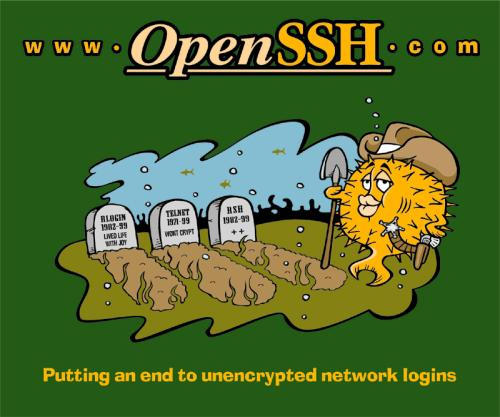
\includegraphics[width=12cm]{images/tshirt-9b.jpg}}  
%\end{center}

\hlkimage{16cm}{images/openssh-banner.png}

\begin{list1}
\item Hvad er Secure Shell SSH?  
\item Oprindeligt udviklet af Tatu Ylonen i Finland,\\
se \link{http://www.ssh.com}
\item SSH afløser en række protokoller som er usikre:
  \begin{list2}
  \item Telnet til terminal adgang
  \item r* programmerne, rsh, rcp, rlogin, ...
  \item FTP med brugerid/password
  \end{list2}
\end{list1}



\slide{Do NOT USE FTP}
\begin{list1}
\item File Transfer Protocol - filoverførsler
\item FTP bruges især til:
  \begin{list2}
    \item FTP - drivere, dokumenter, rettelser - Windows Update? er
    enten HTTP eller FTP
\item Opdatering af websites
\item Overførsel af data mellem virksomheder
\item Serveren er indbygget i de fleste serveroperativsystemer
  \end{list2}
\item FTP sender i klartekst\\ 
{\bfseries USER brugernavn} og \\
{\bfseries PASS hemmeligt-kodeord} 
\end{list1}

\slide{Grafisk Secure Copy - WinSCP}

\begin{center}
\colorbox{white}{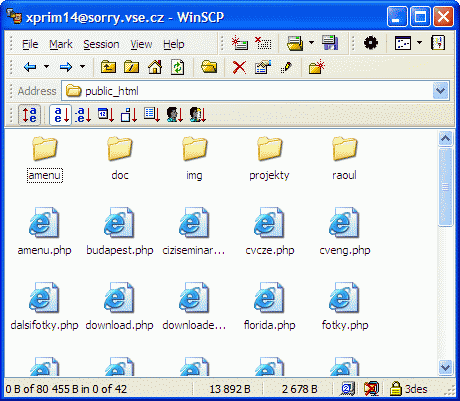
\includegraphics[width=10cm]{images/winscp-explorer.png}}  
\end{center}

\begin{center}
\item benytter Secure Shell protkollen (SSH) 
\item screenshot fra
  \link{http://winscp.vse.cz/eng/screenshots/large/explorer.gif} 
\end{center}


\slide{Filetransfer programs FileZilla - SFTP}

\hlkimage{19cm}{filezilla.png}

\begin{list1}
\item Stop using FTP! Dammit!
\item Lots of programs support SFTP and SCP for secure copying of data
\item \link{http://filezilla-project.org/}
\end{list1}




\slide{Simple Network Management Protocol}

\begin{list1}
\item SNMP er en protokol der supporteres af de fleste professionelle
  netværksenheder, såsom switche, routere
\item hosts - skal slås til men følger som regel med
\item SNMP bruges til: 
  \begin{list2}
    \item \emph{network management}
    \item statistik
    \item rapportering af fejl - SNMP traps
  \end{list2}
\item {\bfseries sikkerheden baseres på community strings der sendes
    som klartekst ...}
\item det er nemmere at brute-force en community string end en
  brugerid/kodeord kombination
\end{list1}

\slide{brute force}

\begin{list1}
\item hvad betyder bruteforcing?\\
afprøvning af alle mulighederne
\end{list1}

\begin{alltt}
\small
Hydra v2.5 (c) 2003 by van Hauser / THC <vh@thc.org>
Syntax: hydra [[[-l LOGIN|-L FILE] [-p PASS|-P FILE]] | [-C FILE]] 
[-o FILE] [-t TASKS] [-g TASKS] [-T SERVERS] [-M FILE] [-w TIME] 
[-f] [-e ns] [-s PORT] [-S] [-vV] server service [OPT]

Options:
  -S        connect via SSL
  -s PORT   if the service is on a different default port, define it here
  -l LOGIN  or -L FILE login with LOGIN name, or load several logins from FILE
  -p PASS   or -P FILE try password PASS, or load several passwords from FILE
  -e ns     additional checks, "n" for null password, "s" try login as pass
  -C FILE   colon seperated "login:pass" format, instead of -L/-P option
  -M FILE   file containing server list (parallizes attacks, see -T)
  -o FILE   write found login/password pairs to FILE instead of stdout
...  
\end{alltt}


\slide{Formål: sund paranoia}


\hlkimage{10cm}{password-window.png}
\centerline{Opbevaring af passwords}


\slide{January 2013: Github Public passwords?}


\hlkimage{20cm}{github-credentials.png}

 Sources:\\
{\footnotesize\link{https://twitter.com/brianaker/status/294228373377515522}\\
\link{http://www.webmonkey.com/2013/01/users-scramble-as-github-search-exposes-passwords-security-details/}\\
\link{http://www.leakedin.com/}\\
\link{http://www.offensive-security.com/community-projects/google-hacking-database/}
}

\vskip 5mm
\centerline{Use different passwords for different sites, yes - every site!}



\slide{NT hashes}

\begin{list1}
  \item NT LAN manager hash værdier er noget man typisk kan samle op i
  netværk 
\item det er en hash værdi af et password som man ikke burde kunne
  bruge til noget - hash algoritmer er envejs
\item opbygningen gør at man kan forsøge brute-force på 7 tegn ad
  gangen!
\item en moderne pc med l0phtcrack kan nemt knække de fleste password
  på få dage!
\item og sikkert 25-30\% indenfor den første dag - hvis der ingen
  politik er omkring kodeord! 
\item ved at generere store tabeller, eksempelvis 100GB kan man dække
  mange hashværdier af passwords med almindelige bogstaver, tal og
  tegn - og derved knække passwordshashes på sekunder. Søg efter
  rainbowcrack med google
\end{list1}

\slide{l0phtcrack LC4}
\begin{center}
\colorbox{white}{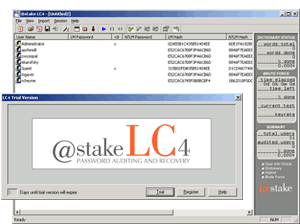
\includegraphics[width=10cm]{images/lc4_splash.png}}  
\end{center}

\begin{alltt}
\small
Consider that at one of the largest technology companies, where policy
required that passwords exceed 8 characters, mix cases, and include
numbers or symbols...   
        
L0phtCrack obtained 18\% of the passwords in 10 minutes         
90\% of the passwords were recovered within 48 hours on a Pentium II/300           
The Administrator and most Domain Admin passwords were cracked 
\link{http://www.atstake.com/research/lc/}
\end{alltt}

\slide{Cain og Abel}

%\hlkimage{10cm}{cain_brute_attack.jpg}
\hlkimage{20cm}{cain-win.png}

\begin{list1}
\item  Cain og Abel anbefales   \link{http://www.oxid.it}
\end{list1}

\slide{John the ripper}

\begin{quote}
John the Ripper is a fast password cracker, currently available for
many flavors of Unix (11 are officially supported, not counting
different architectures), Windows, DOS, BeOS, and OpenVMS. Its primary
purpose is to detect weak Unix passwords. Besides several crypt(3)
password hash types most commonly found on various Unix flavors,
supported out of the box are Kerberos AFS and Windows NT/2000/XP/2003
LM hashes, plus several more with contributed patches.   
\end{quote}

\begin{list1}
\item UNIX passwords kan knækkes med alec Muffets kendte Crack program
  eller eksempelvis John The Ripper \link{http://www.openwall.com/john/}  
\end{list1}

\demo{Cain og Abel}


\slide{Are passwords dead?}

\hlkimage{8cm}{rip-passwords.pdf}

Can we stop using passwords?

Muffett on Passwords has a long list of password related information, from the author of crack \link{http://en.wikipedia.org/wiki/Crack_(password_software)}

\link{http://dropsafe.crypticide.com/muffett-passwords}



\slide{Google looks to ditch passwords for good}

\hlkimage{10cm}{yubico-neo-v1-454x284.jpg}

"Google is currently running a pilot that uses a YubiKey cryptographic card developed by Yubico

The YubiKey NEO can be tapped on an NFC-enabled smartphone, which reads an encrypted one-time password emitted from the key fob."

{\footnotesize Source:
\link{http://www.zdnet.com/google-looks-to-ditch-passwords-for-good-with-nfc-based-replacement-7000010073/}
}



\slide{WEP sikkerhed}

\hlkimage{12cm}{images/airsnort.pdf}  

\begin{quote}
AirSnort is a wireless LAN (WLAN) tool which recovers encryption
keys. AirSnort operates by passively monitoring transmissions,
computing the encryption key when enough packets have been gathered.  

802.11b, using the Wired Equivalent Protocol (WEP), is crippled with
numerous security flaws. Most damning of these is the weakness
described in " Weaknesses in the Key Scheduling Algorithm of RC4 "
by Scott Fluhrer, Itsik Mantin and Adi Shamir. Adam Stubblefield
was the first to implement this attack, but he has not made his
software public. AirSnort, along with WEPCrack, which was released
about the same time as AirSnort, are the first publicly available
implementaions of this attack.  \link{http://airsnort.shmoo.com/}
\end{quote}

%\begin{list1}
%\item i dag er firmware opdateret hos de fleste producenter
%\item men sikkerheden baseres stadig på een delt hemmelighed
%\end{list1}

\slide{major cryptographic errors}

\begin{list1}
\item weak keying - 24 bit er allerede kendt - 128-bit = 104 bit i praksis
\item small IV - med kun 24 bit vil hver IV blive genbrugt oftere
\item CRC-32 som intergritetscheck er ikke \emph{stærkt} nok
  kryptografisk set
\item Authentication gives pad - giver fuld adgang - hvis der bare
  opdages \emph{encryption pad} for en bestemt IV. Denne IV kan så
  bruges til al fremtidig kommunikation
\end{list1}
Source: 
\emph{Secure Coding: Principles and Practices}, Mark G. Graff
  og Kenneth R. van Wyk, O'Reilly, 2003

\slide{Konklusion: Kryptografi er svært}

%Stoler vi på de andre autentificeringsmetoder?}
\hlkimage{20cm}{crypto-class.png}

Åbent kursus på Stanford\\
\link{http://crypto-class.org/}

\slide{Kryptering: Cryptography Engineering}

\hlkimage{8cm}{book-ce-150w.jpg}

\emph{Cryptography Engineering} by
Niels Ferguson, Bruce Schneier, and Tadayoshi Kohno
\link{https://www.schneier.com/book-ce.html}

\centerline{Kryptering sikrer fortrolighed og integritet af beskederne}


\slide{Encryption key length}

\hlkimage{19cm}{encryption-crack.png}

Source: \link{http://www.mycrypto.net/encryption/encryption_crack.html}

\slide{WPA cracking med Pyrit}

\begin{quote}
\emph{Pyrit} takes a step ahead in attacking WPA-PSK and WPA2-PSK, the protocol that today de-facto protects public WIFI-airspace. The project's goal is to estimate the real-world security provided by these protocols. Pyrit does not provide binary files or wordlists and does not encourage anyone to participate or engage in any harmful activity. {\bf This is a research project, not a cracking tool.}

\emph{Pyrit's} implementation allows to create massive databases, pre-computing part of the WPA/WPA2-PSK authentication phase in a space-time-tradeoff. The performance gain for real-world-attacks is in the range of three orders of magnitude which urges for re-consideration of the protocol's security. Exploiting the computational power of GPUs, \emph{Pyrit} is currently by far the most powerful attack against one of the world's most used security-protocols. 
\end{quote}

\begin{list1}
\item \link{http://pyrit.wordpress.com/about/} 
\item Also check out the Reaver brute force WPS\\ \link{https://code.google.com/p/reaver-wps/}
\end{list1}

\slide{ Wi-Fi Protected Setup, WPS hacking - Reaver}

\begin{quote}
How Reaver Works
Now that you've seen how to use Reaver, let's take a quick overview of how Reaver works. The tool takes advantage of a vulnerability in something called Wi-Fi Protected Setup, or WPS. It's a feature that exists on many routers, intended to provide an easy setup process, and it's tied to a PIN that's hard-coded into the device. Reaver exploits a flaw in these PINs; the result is that, with enough time, it can reveal your WPA or WPA2 password.
\end{quote}

\centerline{Hvad betyder ease of use?}

Source: \\
\link{https://code.google.com/p/reaver-wps/}\\
{\footnotesize \link{http://lifehacker.com/5873407/how-to-crack-a-wi+fi-networks-wpa-password-with-reaver}}

\slide{WPS Design Flaws used by Reaver }

\hlkimage{22cm}{wps-design-flaw-1.png}

\centerline{Pin only, no other means necessary}

Source:\\
\link{http://sviehb.files.wordpress.com/2011/12/viehboeck_wps.pdf}



\slide{WPS Design Flaws used by Reaver }

\hlkimage{14cm}{wps-design-flaw-2.png}

\centerline{Reminds me of NTLM cracking, crack parts independently}

Source:\\
\link{http://sviehb.files.wordpress.com/2011/12/viehboeck_wps.pdf}




\slide{Cracking passwords}

\begin{list2}
\item Hashcat is the world's fastest CPU-based password recovery tool.
\item oclHashcat-plus is a GPGPU-based multi-hash cracker using a brute-force attack (implemented as mask attack), combinator attack, dictionary attack, hybrid attack, mask attack, and rule-based attack.
\item oclHashcat-lite is a GPGPU cracker that is optimized for cracking performance. Therefore, it is limited to only doing single-hash cracking using Markov attack, Brute-Force attack and Mask attack.
\item John the Ripper password cracker old skool men stadig nyttig
\end{list2}

Source:\\
\link{http://hashcat.net/wiki/}\\
\link{http://www.openwall.com/john/}

\slide{Parallella John}

\hlkimage{20cm}{parallella-john.png}

\link{https://twitter.com/solardiz/status/492037995080712192}

Warning: FPGA hacking - not finished part of presentation

\slide{Stacking Parallella boards}
\hlkimage{16cm}{4BoardStack.jpg}

\link{http://www.parallella.org/power-supply/}


%\slide{Improving your cryptography configurations}

\slide{Bettercrypto.org}

\hlkimage{20cm}{bettercrypto-nginx.png}
\begin{quote}
Overview

This whitepaper arose out of the need for system administrators to have an updated, solid, well researched and thought-through guide for configuring SSL, PGP, SSH and other cryptographic tools in the post-Snowden age. ... This guide is specifically written for these system administrators. 
\end{quote}

\link{https://bettercrypto.org/}


\slide{Are your data secure - data at rest}

\hlkimage{15cm}{images/data-integrity-1.pdf}

\begin{list1}
\item Stolen laptop, tablet, phone - can anybody read your data?
\item Do you trust "remote wipe"
\item How do you in fact wipe data securely off devices, and SSDs?
\item Encrypt disk and storage devices before using them in the first place!
\end{list1}


\slide{Circumvent security - single user mode boot}
\begin{list1}
\item Unix systems often allows boot into singleuser mode\\
press command-s when booting Mac OS X 
\item Laptops can often be booted using PXE network or CD boot
\item Mac computers can become a Firewire disk\\
hold t when booting - firewire target mode
\item Unrestricted access to un-encrypted data
\item Moving hard drive to another computer is also easy
\end{list1}
\pause
\centerline{Physical access is often - {\bf game over}}


\slide{Encrypting hard disk}

\hlkimage{17cm}{images/apple-filevault.png}

\begin{list1}
\item Becoming available in the most popular client operating systems
\begin{list2}
\item Microsoft Windows Bitlocker - requires Ultimate or Enterprise
\item Apple Mac OS X - FileVault og FileVault2
\item FreeBSD GEOM og GBDE - encryption framework
\item Linux distributions like Ubuntu ask to encrypt home dir during installation
\item PGP disk - Pretty Good Privacy - makes a virtuel krypteret disk
\item TrueCrypt - similar to PGP disk, a virtual drive with data, cross platform
\item Some vendors have BIOS passwords, or disk passwords
\end{list2}
\end{list1}



\slide{Attacks on disk encryption}

\begin{list1}
\item Firewire, DMA \& Windows, Winlockpwn via FireWire\\
Hit by a Bus: Physical Access Attacks with Firewire Ruxcon 2006
\vskip 5mm
\item Removing memory from live system - data is not immediately lost, and can be read under some circumstances\\
Lest We Remember: Cold Boot Attacks on Encryption Keys\\
\link{http://citp.princeton.edu/memory/}
\item This is very CSI or Hollywoord like - but a real threat 
\item VileFault decrypts encrypted Mac OS X disk image files\\ \link{https://code.google.com/p/vilefault/}

\item  FileVault Drive Encryption (FVDE) (or FileVault2) encrypted volumes\\
\link{https://code.google.com/p/libfvde/}
\end{list1}

\centerline{So perhaps use both hard drive encryption AND turn off computer after use?}

\slide{... and deleting data}

\hlkimage{14cm}{dban-screenshot.png}

\begin{list1}
\item Getting rid of data from old devices is a pain
\item Some tools will not overwrite data, leaving it vulnerable to recovery
\item Even secure erase programs might not work on SSD - due to reallocation of blocks
\item I have used Darik's Boot and Nuke ("DBAN") \link{http://www.dban.org/}
\end{list1}





\slide{Backup}

\vskip 3cm
\centerline{\LARGE \bf Kom igang!}

\begin{list2}
\item Skriv på DVD - DVD brændere i mange laptops idag
\item Gem på netværket - Dropbox, husk en yderligere backup!
\item Brug Duplicity på egen server, eller tilsvarende services
\end{list2}

Mat Honan epic hacking :-(\\ {\small\link{http://www.wired.com/gadgetlab/2012/08/apple-amazon-mat-honan-hacking/all/}}

\slide{Duplicity}

\begin{quote}
{\large\bf What is it?}

Duplicity backs directories by producing encrypted tar-format volumes and uploading them to a remote or local file server. Because duplicity uses librsync, the incremental archives are space efficient and only record the parts of files that have changed since the last backup. Because duplicity uses {\bf GnuPG} to encrypt and/or sign these archives, they will be safe from spying and/or modification by the server.
\end{quote}

\link{http://duplicity.nongnu.org/} duplicity home page

\link{http://www.gnupg.org/} The GNU Privacy Guard



\slide{Sikkerhedsteknologier}

\begin{list1}
\item Brug alt hvad I kan overkomme:
\begin{list2}
\item Firewalls: IPfilter, IPtables, OpenBSD PF
\item Kryptografi 
\item Secure Shell - SSH
\item betragt Telnet, Rlogin, Rsh, Rexec som døde!
\item FTP bør kun bruges til anonym FTP
\item Intrusion Detection - Snort
\item Sudo
\item Tripwire, mtree, MD5
\end{list2}
\item Sikkerhedspolitikken er din "plan" for sikkerheden
- og er med til at sikre niveauet er ens
\item Firewalls hjælper ikke mod alle trusler
\end{list1}






% opsummering


\slide{Basic tools - PGP}

\hlkimage{5cm}{images/pgp.png}

\begin{list2}
\item Pretty Good Privacy - PGP 
\item Originally developed by Phil Zimmermann 
\item Now a commecrial entity \link{http://www.pgp.com}
\item Source exported from USA on paper and scanned outside - which was legal 
\item \link{http://www.pgpi.org}
\end{list2}


\slide{Basic tools - GPG}

\hlkimage{5cm}{images/logo-gnupg.png}
\begin{list1}
\item Gnu Privacy Guard, GnuPG or GPG
\item Web site:
  \link{http://www.gnupg.org/}
\item Open Source - GPL license 
\item Available for most popular operating systems
\item Highly recommended
\end{list1}


\slide{GnuPG - verifikation af downloads}

\begin{alltt}
\small
$ cd /userdata/download/src/postfix/
$ ls -l *.sig 
-rw-r--r--  1 hlk  admin  152 13 Sep  2003 postfix-2.0.16.tar.gz.sig
-rw-r--r--  1 hlk  admin  152  3 May 13:34 postfix-2.1.1.tar.gz.sig
$ {\bf gpg --verify postfix-2.1.1.tar.gz.sig} 
gpg: Signature made Mon May  3 19:34:08 2004 CEST using RSA key ID D5327CB9
gpg: {\bf Good signature} from "wietse venema \verb+<wietse@porcupine.org>+"
gpg:                 aka "wietse venema <wietse@wzv.win.tue.nl>"
$
\end{alltt}

\begin{list1}
\item {\bf Det er nødvendigt at verificere arkiver med kildekode!}  
\end{list1}



\slide{Enigmail - GPG plugin til Mail}

\hlkimage{20cm}{images/enigmail-compose}
\begin{list2}
\item Enigmail is a plugin for the Thunderbird mail client
\item Screenshot from \link{http://enigmail.mozdev.org}
\end{list2}


\slide{Enigmail - OpenGPG Key Manager}

\hlkimage{18cm}{images/enigmail-keyman1}

\vskip 1cm
\centerline{Key Manager built-int Enigmail is recommended}  

\slide{Generering af keys 1}

\begin{list1}
\item Generering af key
\begin{alltt}
\$ gpg --gen-key
\end{alltt}
\begin{list2}
  \item Vælg "DSA and Elgamal"
  \item Vælg passende keysize - 4096 skader næppe
  \item Vælg passende udløbsdato - "no expire" vil virke for de fleste
  \item Brug din officielle mailaddresse i forbindelse med dit navn, så 
        Email klienter kan finde din key aytomatisk
  \item Brug en god passphrase. \\
        En lang sætning som du kan huske, og som ikke kan gættes udfra
        kendskab til dig.
  \item Når nøglen genereres, så hjælp med at generere "randomness" i systemet.
        Det får genereringen til at gå hurtigere, og det giver en bedre key.
\end{list2}

\item samme spørgsmål i GUI programmerne, {\bf og husk at lave et revoke certifikat!}
\end{list1}

\slide{Generering af keys 2}

\begin{list1}
\item Du har nu en GnuPG key klar til at blive signeret
\item Er du {\bf sikker} på at du kan huske din passphrase?
\item Når nøglen er genereret bliver der vist et kort sammendrag af 
      indholdet\\
      Dette \emph{fingerprint} kan også fås frem med:
\end{list1}

\begin{alltt}
\small
$ gpg --fingerprint addr@domain.dk
pub   1024D/D1EFBAA6 2003-01-20
      Key fingerprint = 0FAE F19D DB46 DF2E D93D  9B05 21A6 469B D1EF BAA6
uid                  Henrik Lund Kramshoej (work email) <hlk@security6.net>
uid                  Henrik Lund Kramshoej (Kramse) <hlk@kramse.dk>
uid                  [jpeg image of size 14412]
sub   2048g/6D08E6E6 2003-01-20
\end{alltt}
%$

\slide{Signering af keys}
\begin{list1}
\item Keys signeres med: \\
\begin{alltt}
gpg --sign-key addr@domain.dk  \# Eller keyid
\end{alltt}
\item Husk at sikre at det nu også er den korrekte key i signerer \\
      Kontroller med: \\
\begin{alltt}
gpg --fingerprint addr@domain.dk
\end{alltt}
\end{list1}

\slide{GPGMail plugin for Mac OS X Mail.app}

\hlkimage{20cm}{images/gpgmail-new-message.png}      

\begin{list2}
\item Uses GPG and is part of the GPGTools
\item \link{https://gpgtools.org/}
\end{list2}


\slide{Email er usikkert}

\hlkimage{20cm}{email-uden-krypterin.png}

\centerline{Email uden kryptering - er som et postkort}



\slide{Email med kryptering - afsendelse}

\hlkimage{18cm}{email-med-kryptering.png}


\centerline{En sikker krypteret email er ikke sværere at sende}

\slide{Krypteret Email under transporten}

\hlkimage{11cm}{modtaget-email-med-kryptering.png}

\centerline{En sikker krypteret email er beskyttet undervejs}


\slide{Crypto Projects that Might not Suck}
Steve Weis\\
PrivateCore\\
!
\link{http://bit.ly/CryptoMightNotSuck}

\slide{VPN}

\hlkimage{12cm}{openvpn-gui-systray.png}

\begin{list1}
\item Virtual Private Networks are useful - or even required when travelling
\item VPN \link{http://en.wikipedia.org/wiki/Virtual_private_network}
\item SSL/TLS VPN - Multiple incompatible vendors: OpenVPN, Cisco, Juniper, F5 Big IP
\item IETF IPsec does work cross-vendors - sometimes, and is also increasingly becoming blocked or unusable due to NAT :-(
\item Recommended starting point OpenVPN - free and open, clients for "anything"
\end{list1}


\slide{Turkey: Erdogan bans Twitter }

\hlkimage{12cm}{twitter-turkey.png}

\slide{Censorship on the internet - lol}

\centerline{\color{titlecolor} The Net interprets censorship as damage and routes around it.}

\hlkimage{22cm}{John-Gilmore-quotes.png}

\link{http://en.wikiquote.org/wiki/John_Gilmore}\\
\link{http://en.wikipedia.org/wiki/John_Gilmore_(activist)}

\slide{Directly connection Tor Users from Turkey}

\hlkimage{20cm}{userstats-relay-country-2013-12-25-off-2014-03-25-tr.png}

Image from \link{https://metrics.torproject.org}\\
via \link{https://twitter.com/runasand}

\slide{Directly connection Tor Users from Turkey +10.000}

\hlkimage{20cm}{userstats-relay-country-2013-12-25-off-2014-03-26-tr.png}

Image from \link{https://metrics.torproject.org} via 
\link{https://twitter.com/ioc32/status/448791582423408640}


\slide{Tor project}

\hlkimage{21cm}{tor-project.png}

\centerline{\link{https://www.torproject.org/}}

\slide{Tor project - how it works 1}

\hlkimage{21cm}{how-tor-works-1.png}

\centerline{pictures from \link{https://www.torproject.org/about/overview.html.en}}

\slide{Tor project - how it works 2}

\hlkimage{21cm}{how-tor-works-2.png}

\centerline{pictures from \link{https://www.torproject.org/about/overview.html.en}}

\slide{Tor project - how it works 3}

\hlkimage{21cm}{how-tor-works-3.png}

\centerline{pictures from \link{https://www.torproject.org/about/overview.html.en}}




\slide{Tor project install}

\hlkimage{12cm}{tor-project.png}

Der findes diverse tools til Tor, Torbutton on/off knap til Firefox osv.

Det anbefales at bruge Torbrowser bundles fra \link{https://www.torproject.org/}

\slide{Torbrowser - anonym browser}

\hlkimage{20cm}{torbrowser-main-window.png}

\centerline{\color{titlecolor} Mere anonym browser - Firefox in disguise}

\slide{Whonix - Tor to the max!}

\hlkimage{17cm}{400px-Whonix.jpg}

\begin{quote}
Whonix is an operating system focused on anonymity, privacy and security. It's based on the Tor anonymity network[5], Debian GNU/Linux[6] and security by isolation. DNS leaks are impossible, and not even malware with root privileges can find out the user's real IP. \link{https://www.whonix.org/}

\end{quote}

\centerline{Torbrowser er godt, Whonix giver lidt ekstra sikkerhed}

\slide{Torbrowser - sample site}

\hlkimage{18cm}{sample-tor-site.png}

\centerline{\color{titlecolor} .onion er Tor adresser - hidden sites}

{\footnotesize Den viste side er SecureDrop hos Radio24syv \link{http://www.radio24syv.dk/dig-og-radio24syv/securedrop/}}

\slide{SecureDrop}

\hlkimage{8cm}{sample-tor-site.png}

Even if you dont want to use SD specifically, look at the technologies used.
\begin{list2}
\item Hidden services with authentication key
\item Jails/chroot/compartmented data
\item AppArmor 
\item Google Authenticator
\item Host based IDS, monitoring server
\end{list2}




\slide{Multiple browsers}

\hlkimage{20cm}{multi-browser-strategy.png}

\begin{list2}
\item Strict Security settings in the general browser, Firefox or Chrome?
\item More lax security settings for "trusted sites" - like home banking
\item Security plugins like HTTPS Everywhere and NoScripts for generic browsing
\end{list2}

\slide{HTTPS Everywhere}

\hlkimage{5cm}{HTTPS_Everywhere_new_logo.jpg}
\begin{quote}
HTTPS Everywhere is a Firefox extension produced as a collaboration between The Tor Project and the Electronic Frontier Foundation. It encrypts your communications with a number of major websites.
\end{quote}

\centerline{\link{http://www.eff.org/https-everywhere}}

\slide{DNSSEC trigger}

\hlkimage{7cm}{dnssec-trigger.png}

Lots of DNSSEC tools, I recommend DNSSEC-trigger a local name server for your laptop

\begin{list2}
\item DNSSEC Validator for firefox\\ \link{https://addons.mozilla.org/en-us/firefox/addon/dnssec-validator/}
\item OARC tools \link{https://www.dns-oarc.net/oarc/services/odvr}
\item \link{http://www.nlnetlabs.nl/projects/dnssec-trigger/}
\end{list2}


\slide{DANE}

\begin{quote}
Objective:

Specify mechanisms and techniques that allow Internet applications to
establish cryptographically secured communications by using information
distributed through DNSSEC for discovering and authenticating public 
keys which are associated with a service located at a domain name.
\end{quote}

DNS-based Authentication of Named Entities (dane)\\
\link{https://datatracker.ietf.org/wg/dane/charter/}\\
{\footnotesize \link{http://googleonlinesecurity.blogspot.dk/2011/04/improving-ssl-certificate-security.html}}

\vskip 2cm

\centerline{\Large DNSSEC er ved at være godt udbredt - undtagen i DK}
(findes på .dk zonen, men næsten ingen resolvere)

\slide{www.uncensoreddns.org}

\hlkimage{20cm}{censurfridns-1.png}






%\slide{}

%Security for Journalists, via Silkie Carlo






\slide{Secure your mobile}

\hlkimage{20cm}{the-guardian-project.pdf}

\centerline{Dont forget your mobile platforms \link{https://guardianproject.info/}}


\slide{24 Deadly Sins of Software Security}

\hlkrightimage{5cm}{24-deadly.jpg}
\emph{24 Deadly Sins of Software Security} af Michael Howard, David Leblanc, John Viega 2009

\begin{list1}
\item {\bf Obligatorisk læsning for alle udviklere}
\item Denne bog er præcis og giver overblik på kun 432 sider
\item Buffer Overruns, Format String Problems, Integer Overflows, SQL Injection, Command Injection,
Failing to Handle Errors, Cross-Site Scripting, Failing to Protect Network Traffic, Magic URLs Hidden Form Fields,
Improper Use of SSL and TLS, Weak Password-Based Systems, Failing to Store and Protect Data Securely, Information
Leakage, Improper File Access, Trusting Network Name Resolution, Race Conditions, Unauthenticated Key Exchange, Cryptographically Strong Random Numbers, Poor Usability 
\end{list1}


\slide{Open Mike night ...}

\vskip 3 cm

\centerline{\Large Hvad glemte jeg? Kom med dine favoritter \smiley}

evalg, DNS censur, NemID bashing, malware sucks, Android malware, iPhone malware?

Did you notice how a lot of the links in this presentation uses HTTPS - encrypted


\myquestionspage



\slide{Reklamer: kursusafholdelse}

\begin{list1}
\item Følgende kurser afholdes med mig som underviser
\begin{list2}
\item IPv6 workshop - 1 dag\\
 Introduktion til Internetprotokollerne og forberedelse til
  implementering i egne netværk. 
\item Wireless teknologier og sikkerhed workshop - 1-2 dage\\
En dag med fokus på netværksdesign og fornuftig implementation af
trådløse netværk, samt integration med hjemmepc og
wirksomhedsnetværk. 
\item Hacker workshop 2 dage\\
Workshop med detaljeret gennemgang af hackermetoderne angreb over
netværk, exploitprogrammer, portscanning, Nessus m.fl.
\item Forensics workshop 2 dage\\
Med fokus på tilgængelige open source værktøjer gennemgås metoder og
praksis af undersøgelse af diskimages og spor på computer systemer
\item Moderne Firewalls og Internetsikkerhed 2 dage\\
Informere om trusler og aktivitet på Internet, samt give et bud
på hvorledes en avanceret moderne firewall idag kunne konfigureres.
\end{list2}
\end{list1}


\end{document}
